\documentclass[pdftex,twocolumn,10pt,letterpaper]{article}
\usepackage{graphicx, times}
\usepackage{wrapfig}
\graphicspath{{figures/}}

\setlength{\textheight}{9.0in}
\setlength{\columnsep}{0.25in}
\setlength{\textwidth}{6.50in}
\setlength{\topmargin}{0.0in}
\setlength{\headheight}{0.0in}
\setlength{\headsep}{0.0in}

\begin{document}

\title{ Comparative Analysis of Stream Processing Systems }
\author{
    Shawn Zhong, Suyan Qu, Sulong Zhou \\
    \{wzhong36, squ27, szhou78\}@wisc.edu\\
    \\
    CS 744: Big Data Systems \\
    Group No. 7
}
\date{October 17, 2019}

\interfootnotelinepenalty=10000

\maketitle

\section{Introduction}
The explosion of modern information and computer science technology systems has extremely accelerated the development of data science. The ubiquitous social network, e-commerce platform and search engine continuously produce steady flows of high-volume data\cite{mcafee2012big}. Meanwhile, handling and analyzing real-time big data have become core demands for business and industry. This dramatic escalation in volumes of stream data is challenging existing data processing systems because of the high-volume of users, low-latency of processing, heterogeneous resources, and burstiness of events.  

In order to deal with the emerged challenges from 3 major perspectives (volume, velocity, and variety) of stream data\cite{birke2014big}, and satisfy the needs of related markets, many stream data processing platforms targeted in scalability, fault tolerance, and computing speed have been developed and deployed, such as Twitter’s Heron~\cite{Kulkarni:2015:THS:2723372.2742788}, Twitter's Storm \cite{toshniwal2014storm}, LinkedIn’s Samza~\cite{Noghabi:2017:SSS:3137765.3137770}, and Apache Flink~\cite{Carbone2015ApacheFS}. Meanwhile, a lot of efforts have been put into how to evaluate the performance of these frameworks when dealing with stream data. 

Theoretically and practically, benchmark rises in response to evaluate the performance of these frameworks. Considering the fast speed of the invention and development of the stream data processing systems, a set of universal standards is required to provide accurate, comprehensive, and uniformed measurement across the diversity of stream data processing frameworks. 

In this work, we propose a review of current efficient standards for 5 different stream data processing frameworks. The standards are not only based on technique workflow and metrics, such as task scheduling, resource utilization, data processing model, fault toleration, scalability, throughput, and latency, but also social parameters, such as community engagement and user inclusion.



\section{Background}

\subsection{Stream Processing}
Big data computing models are mainly divided into batch computing, stream computing, interactive computing, graph computing, etc. Among them, stream computing and batch computing are two main big data computation modes, which apply to different big data application scenarios. 

Streaming data (or data stream) refers to a series of dynamic data that comes indefinitely. The value of data decreases with time, so it must be calculated in real-time to give a response in seconds. 

Streaming processing, as its name implies, is the processing of data streams, which is a real-time calculation. Batch calculation is a method of uniformly collecting data, storing it in a database, and then performing batch processing on the data. 

The difference is mainly reflected in the following aspects: 

\begin{enumerate}
    \item Data timeliness: stream computing requires real-time, low latency, whereas batch computing can tolerate high latency. 
    
    \item Data characteristics: stream data is generally dynamic, there is no boundary, and the batch data is generally static data. 
    
    \item Application scenarios: Streaming computing applications are used in real-time scenarios, where timeliness requirements are relatively high, such as real-time recommendation, business monitoring, etc. Batch computing generally says batch processing, applications in real-time requirements are not high, offline computing scenarios, data analysis, offline reports, and more. 
    
    \item Execution method: The task of stream computing is continuous, and the task of batch computing is completed at one time.
\end{enumerate}

\subsection{Stream Processing Systems}

\subsubsection{Apache Storm}
Apache Storm is Twitter's first generation of real-time fault-tolerant stream data processing system. In Storm, tasks are handled on a master node called Nimbus. It communicates with a set of Zookeepers\cite{hunt2010zookeeper} that monitors the supervisors of a set of worker nodes. Storm does not have any data structure for storage. Data storage is handled by external data management systems such as Hadoop File System\cite{shvachko2010hadoop}. 

\subsubsection{Apache Heron}
Heron is the second-generation real-time stream data processing system used in Twitter improved from Apache Storm. In Storm, each worker runs multiple threads for different jobs, leading to no resource isolation between different jobs. Heron improves by replacing Nimbus by an external scheduler such as Aurora\cite{abadi2003aurora}, which can provide more resource isolation. In addition, in Heron, the scheduler no longer communicates with Zookeepers for workers' heartbeats and task assignments. Instead, it communicates with Topology Masters for task assignment, while a separate monitoring system will manage the server status, resource usage, and other related metrics for failure recovery and performance improvement. 

\subsubsection{Spark Streaming}

Spark Streaming is an extension of the Spark core API that enables high-throughput, fault-tolerant real-time streaming data processing. In Spark Streaming, Master is mainly responsible for overall cluster resource management and application scheduling; Worker is responsible for resource management of a single node (startup of drivers and executors, etc); Driver is the place where the user entry program is executed, which includes DAG generation, stage division, task generation, and scheduling; Executors are responsible for executing tasks, feedback execution status and execution results.

\subsubsection{Apache Flink}

Apache Flink is a distributed processing engine for streaming data and batch data. The stream-first approach provides low latency, high throughput, per-item processing, and the ability to compute complex calculations. Flink integrates with all common cluster resource managers such as Hadoop YARN\cite{vavilapalli2013apache}, Apache Mesos\cite{hindman2011mesos}, and Kubernetes\cite{burns2016borg} but can also be setup to run as a stand-alone cluster by resource-manager-specific deployment modes. Low latency is guaranteed by local state optimization in memory. Flink applications are parallelized in a distributed system. Therefore, an application can leverage virtually unlimited amounts of CPUs, main memory, disk, and network IO. 

\subsubsection{Apache Kafka \& Kafka Streams}

Kafka\cite{kreps2011kafka} was originally developed by Linkedin. It is a distributed, partitioned, replica, distributed messaging system based on Zookeeper. Its biggest feature is that it can process large amounts of data in real time to meet various workload scenarios: such as Hadoop-based batch processing systems, low-latency real-time systems, web logs, access logs, message services, etc. \\

Kafka Streams is a real-time stream computing library that relies on existing Kafka clusters to provide distributed, highly fault-tolerant, real-time stream computation. Kafka Streams is designed to be lightweight. It has no external dependencies other than Kafka Stream Client library and can be easily embedded in Java applications. 

\section{Comparisons}

\begin{figure*}[!ht]
    \centering
    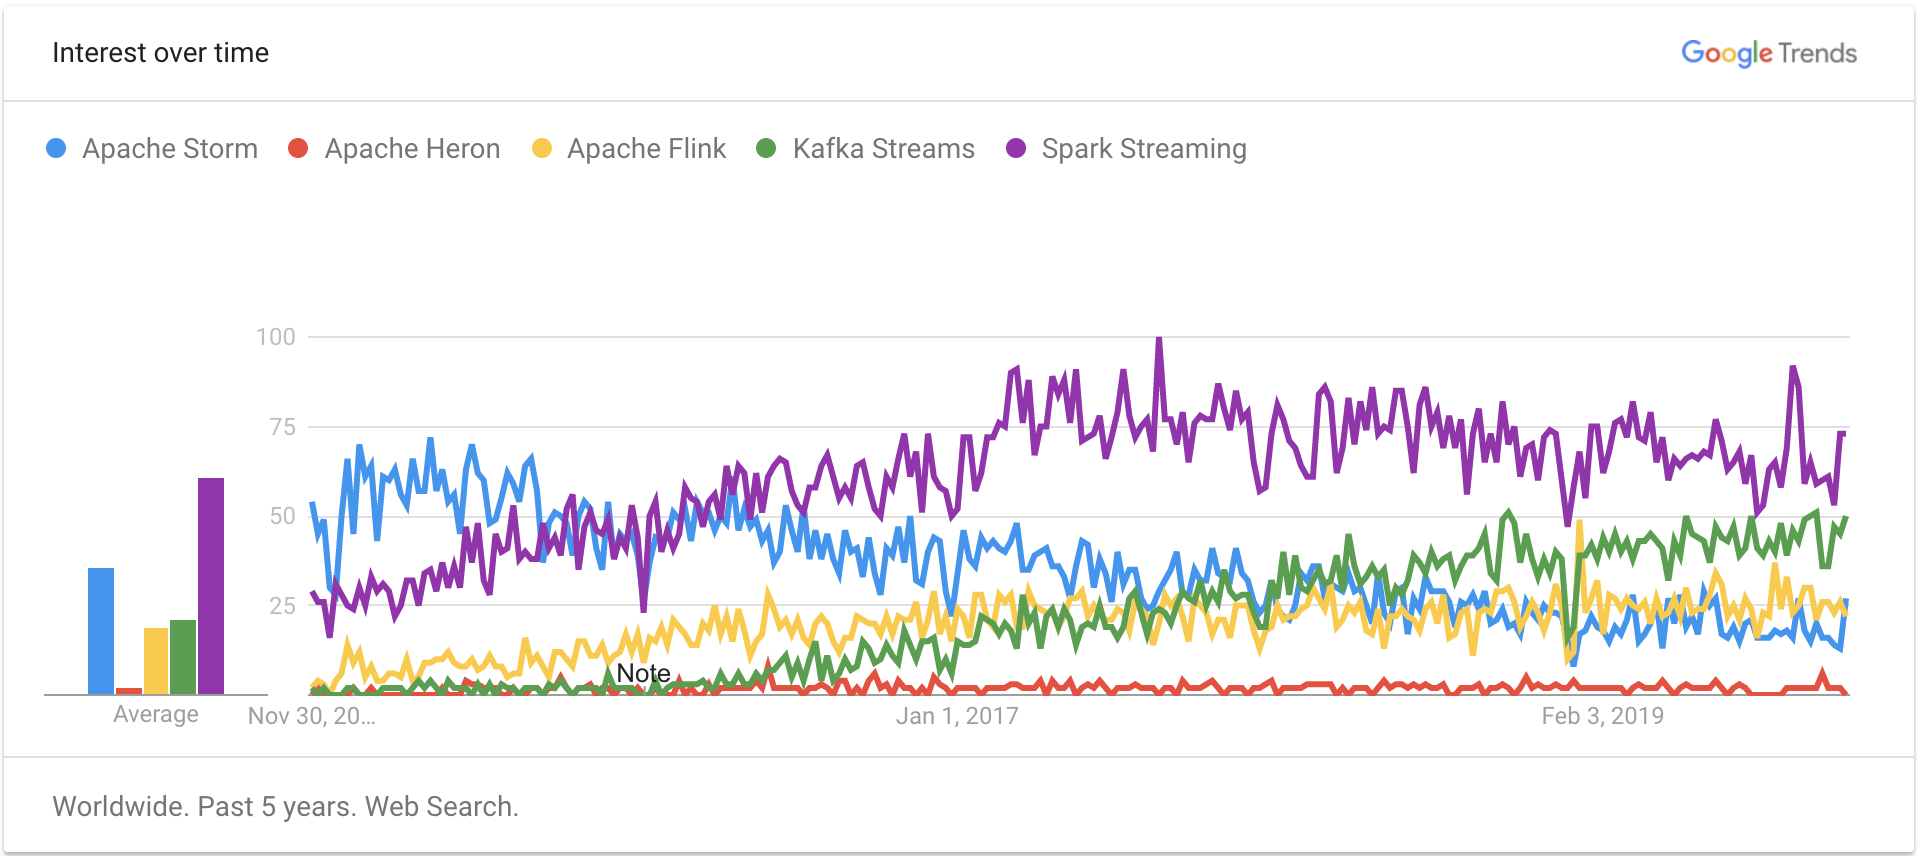
\includegraphics[width=\textwidth]{trend.png}
    \caption{Google search trends\cite{googletrend} for different stream processing systems over the past 5 years.}
    \label{fig:trend}
\end{figure*}

\subsection{Computation Model}
Stream processing systems nowadays typically follow Dataflow model\cite{Dataflow}, where data are grouped into batches by their event time and processed based on processing time when the streaming system starts to process them. How exactly data are batched and how to handle late data varies widely among different stream processing systems. 

In Apache Storm and Heron, the computation graph is called topology. After the user designing a topology, it is then submitted to the cluster, where the master node is responsible for allocating code to the worker nodes, and the worker nodes are responsible for executing the code. There are two roles in a topology: spout and bolt. Data is passed between spouts, which send data streams as tuples, and bolts are responsible for converting data streams.

Spark Streaming is an extension of the core Spark API. Unlike Storm, it does not process a single stream of data at the same time. Instead, it splits the data stream by time interval before processing the data stream. The abstraction for continuous data streams in Spark Streaming is called DStream (Discretized Stream), which is a small batch of RDD (Elastic Distributed Dataset). RDD can be converted by any function and sliding data window for parallel operation.

The basic building blocks of Flink programs are stream and transformation. Stream is an intermediate result data, and transformation is an operation that performs calculation processing on one or more input (e.g., Map, FlatMap, Reduce, Window). When executed, the Flink program is mapped to the data stream, which is composed of the stream and the corresponding transformation. Each data stream starts at one or more sources and ends at one or more sinks (e.g., writeAsText, writeAsCsv, print). Data flow is similar to an arbitrary directed acyclic graph. 

Kafka Streams applications are composed of several stream partitions. A stream partition is defined as an ordered, fault-tolerant, and read-only data queue. Each record is in the form of a key-value pair. Kafka Streams applications define computing logic through several topologies. The nodes in the topology are stream processors, such as map, filter, join, aggregate and other operators; source and sink processors are special cases, identifying the start and end of the topology. The edges are data streams connecting two stream processors.

\subsection{Scalibility}


Kafka Streams is difficult to meet the complex computing requirements of a large amount, and the input and output of the data are dependent on the Kafka cluster. For other data sources, Kafka connect is required to input the data into the Kafka, and then processed by the Kafka Streams program. Therefore, Kafka Streams is more suitable for scenarios where the computational complexity is small and the data flow process is from Kafka to Kafka.

\subsection{Timeliness}
Timeliness refers to how soon after an event happens it will be processed in the streaming system. It involves many factors such as network bandwidth and latency on client and server sides. Here we mainly consider the latency of these stream processing systems. 

Storm, Heron, Flink, Kafka are designed for real-time stream processing. Once the data comes, it is processed. This processing model can significantly reduce latency. For mission-critical services, such as Twitter, low-latency is necessary. However, real-time stream processing poses many additional challenges, such as skipping or repetitively processing the same data during machine restart or job migration for fault tolerance or straggler mitigation. 

Spark Streaming, on the other hand, is micro-batch processing. When a record arrives, Spark Streaming waits for a small amount of time. Any additional records that arrive during this period will be batched and processed together. This design leads to latency higher than real-time stream processing, but batching multiple records allows for high throughput computation and thereby increases efficiency. Its utilization of Resilient Distributed Datasets (RDD)\cite{rdd} also makes it cheap to recover from machine failure. 


\subsection{Social Factors}
\begin{table*}[!ht]
    \centering
    \begin{tabular}{|c|c|c|c|c|c|}
         \hline
          System & 
          Commits Past Year & 
          Committer & 
          Lines of Code &
          Open Issues & 
          Search Index
          \\ 
         \hline
         Apache Storm & 228 & 305 & 377,166 & 1,033 & 10\\ 
         \hline
         Apache Heron & 201 & 106 & 252,322 & 363 & 2\\ 
         \hline
         Spark Streaming & 2,565 & 1451 & 962,336 & 1,859 & 36\\
         \hline
         Apache Flink & 4,312 & 595 & 1,429,183 & 2,913 & 79\\
         \hline
         Kafka Streams & 1,201 & 606 & 459,984 & 2,616 & 23\\
         \hline
    \end{tabular}
    \caption{
        Social factors associated with each stream processing system.
        Note that the statistics of Spark Streaming include Spark, Spark SQL, and other Spark projects.
        Search index is the Google search trend of the framework.
    }
    \label{tab:social}
\end{table*}

In this section, we consider the social influences of different stream processing frameworks. We focus on two areas: Google search history, representing the popularity and trend of these stream processing systems, and repository information (including the number of commits, number of contributors, lines of code and number of open issues), indicating whether the system is actively being developed.

\subsubsection{Trends}

Figure \ref{fig:trend} shows the Google search trend over the past 5 years. It is noticed that Apache Storm was the most popular stream processing system. However, Spark Streaming quickly exceeds Apache Storm, since it is easier to implement and deploy. Spark Streaming also provides cheaper fault tolerance and capability to seamlessly integrate with non-stream processing tasks, while only slightly increase latency. These characteristics make it the most popular stream processing system over the past 3 years. 

On the other hand, we see a steady decreasing trend for Apache Storm. In fact, Twitter is one of the companies that move away from using Storm to Heron in 2015. Yet Heron depends on a wide range of external tools such as Hadoop File System, Aurora, Zookeeper, etc, making it extremely complicated to deploy and implement in a large scale. As a result, it remains the least popular system over the past 5 years. 

It is also worth noting that Apache Kafka is also experiencing a steady increase in popularity, with various companies such as Uber Technology Inc., and Palo Alto Network Inc using it nowadays. 

\subsubsection{Codebase Analysis}

Table \ref{tab:social} also indicates the popularity and sophistication of these stream processing systems. Storm and Heron are smaller projects, with much fewer commits and less open issues than the others, indicating that Storm and Heron are not widely used. On the other hand, Spark and Flink are the two large projects, each with around 1 million lines of code. Yet we notice that Spark has 1,451 contributors but only 2,565 commits in the past year and less than 2,000 issues open. 

In contrast, Apache Flink has over 4000 commits in the past year and almost 3,000 issues open. This indicates that Spark Streaming is relatively sophisticated and easy to use, while Flink is still actively being upgraded, with various supports for other systems such as Mesos, YARN, Kubernetes, etc. 

It is also worth noting that Kafka Streams is designed to be light-weighted, with less than 500,000 lines of code, but it has over a thousand commits in the past year and over 2,600 open issues, comparable with Apache Flink and Spark Streaming. This indicates that Kafka is gaining popularity and is still actively under development. 


\section{Benchmark}

\subsection{Experiment Setup}

We deploy the stream processing system to a single-node cluster on Amazon Web Services in zone us-west-2c using Databricks Community Edition. 

We use Yahoo Benchmarks\cite{7530084} for performance analysis. For event generation, the input data consist of randomly generated user actions with ad clicks. The records have the following schema: 


\begin{figure}
    \centering
    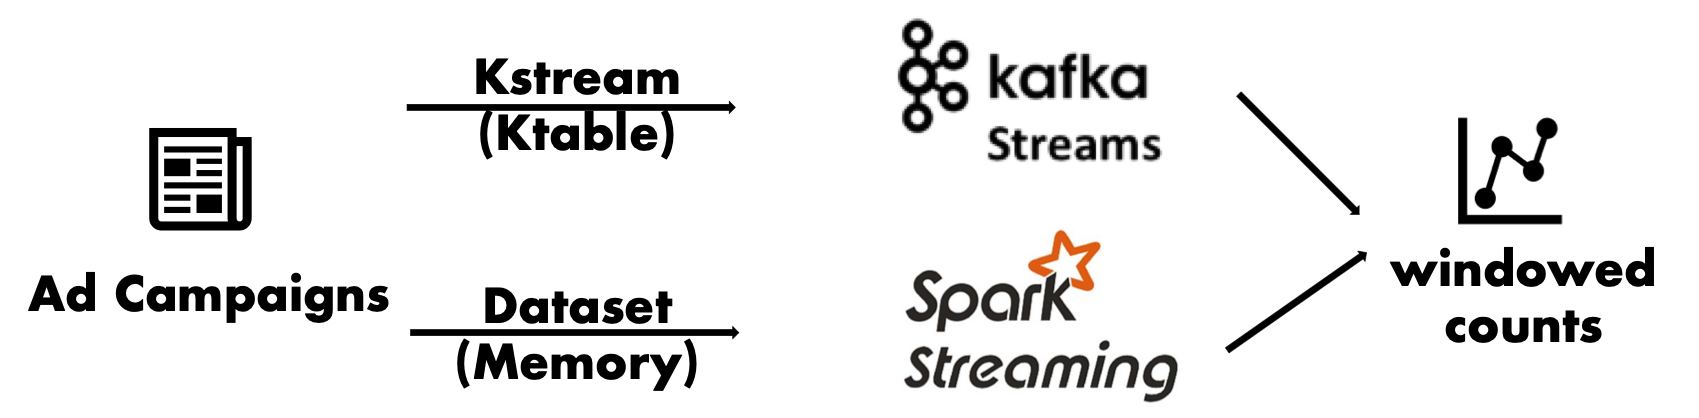
\includegraphics[width=\linewidth]{dataflow.png}
    \caption{Workflow of benchmark process}
    \label{fig:workflow}
\end{figure}

\begin{itemize}
    \item User ID: UUID
    \item Page ID: UUID
    \item Ad ID: UUID
    \item Ad Type: "banner", "modal", "sponsored-search", "mail", or "mobile"
    \item Event Time: Timestamp
    \item Event Type: "view", "click", or "purchase"
    \item IP Address: String
\end{itemize}


The schema stores related information for a number of advertisements promoted by many campaigns. The job of the Yahoo benchmark consists of six operations performed on data streams.

\begin{enumerate}
    \item Read and deserialize event data from Kafka
    \item Filter out irrelevant events based on the Event Type field
    \item Project on Ad ID and Event Time fields
    \item Join each event by Ad ID with its associated Campaign ID
    \item Calculate the windowed count of events per campaign
    \item Write the output for each window back to Kafka along with a timestamp at which the window was last updated
\end{enumerate}

We generate 5,000,000 records per second with ramp-up time of 10 seconds to allow the JVM to warm up. In Kafka Streams, the static table is imported from Kafka as a KTable. In case of a shuffle overhead in Kafka Streams, we equivalently partition the static table and the events stream. In Spark, we join event stream with a static local dataset. The processing system will count the number of actions, such as views, clicks, on each ads. 

The output has the following schema

\begin{itemize}
    \item Time Window: Timestamp
    \item Campaign ID: String
    \item Count: Long
    \item Last Update: Timestamp
\end{itemize}

All versions for the software and libraries used are listed in Table \ref{tab:setup} 

\begin{table}[]
    \centering
    \begin{tabular}{|c|c|c|c|c|c|}
         \hline
         Software / Library & Version \\
         \hline
         Scala & 2.11 \\ 
         \hline
         Apache Kafka & 0.10.2.1 \\ 
         \hline
         Apache Spark & 2.4.4 \\
         \hline
         Databricks runtime & 6.1 \\ 
         \hline
    \end{tabular}
    \caption{Benchmark Environment}
    \label{tab:setup}
\end{table}


\subsection{Benchmark Result}
We run Yahoo Benchmarks on Spark Streaming and Kafka Streams for 5 times. Results are shown in Figure \ref{fig:latency} and Figure \ref{fig:throughput}. 

The latency was calculated in two steps. First, the timestamp of the latest record that was received for a pair of campaign and event-time-window during the windowed counts phase. Second, the latency was indicated by the difference between this timestamp and the Kafka ingestion timestamp of the output. As shown in Figure \ref{fig:latency}, we compared the latency between spark streaming and Kafka streams, the Kafka streams has much higher latency. This is very counter intuitive. Here are some of our proposed explanations: 
\begin{itemize}
    \item Kafka Stream is still a newly-developed, light-weighted stream processing system that is not well optimized for complicated stream computation, such as joining Ads with Campaign ID. 
    \item Kafka Stream is a client-side library, so there might be some communication overhead between the client and the cluster. For Spark Streaming, the user only communicate with the cluster once when they submit the job to the cluster, and the result is saved on the cluster for manual retrieval.  
    \item Kafka creates Kstream / Ktable for streaming data, which may be associated with a large overhead, especially when working with large-scale real-time processing tasks. 
\end{itemize}

\begin{figure}
    \centering
    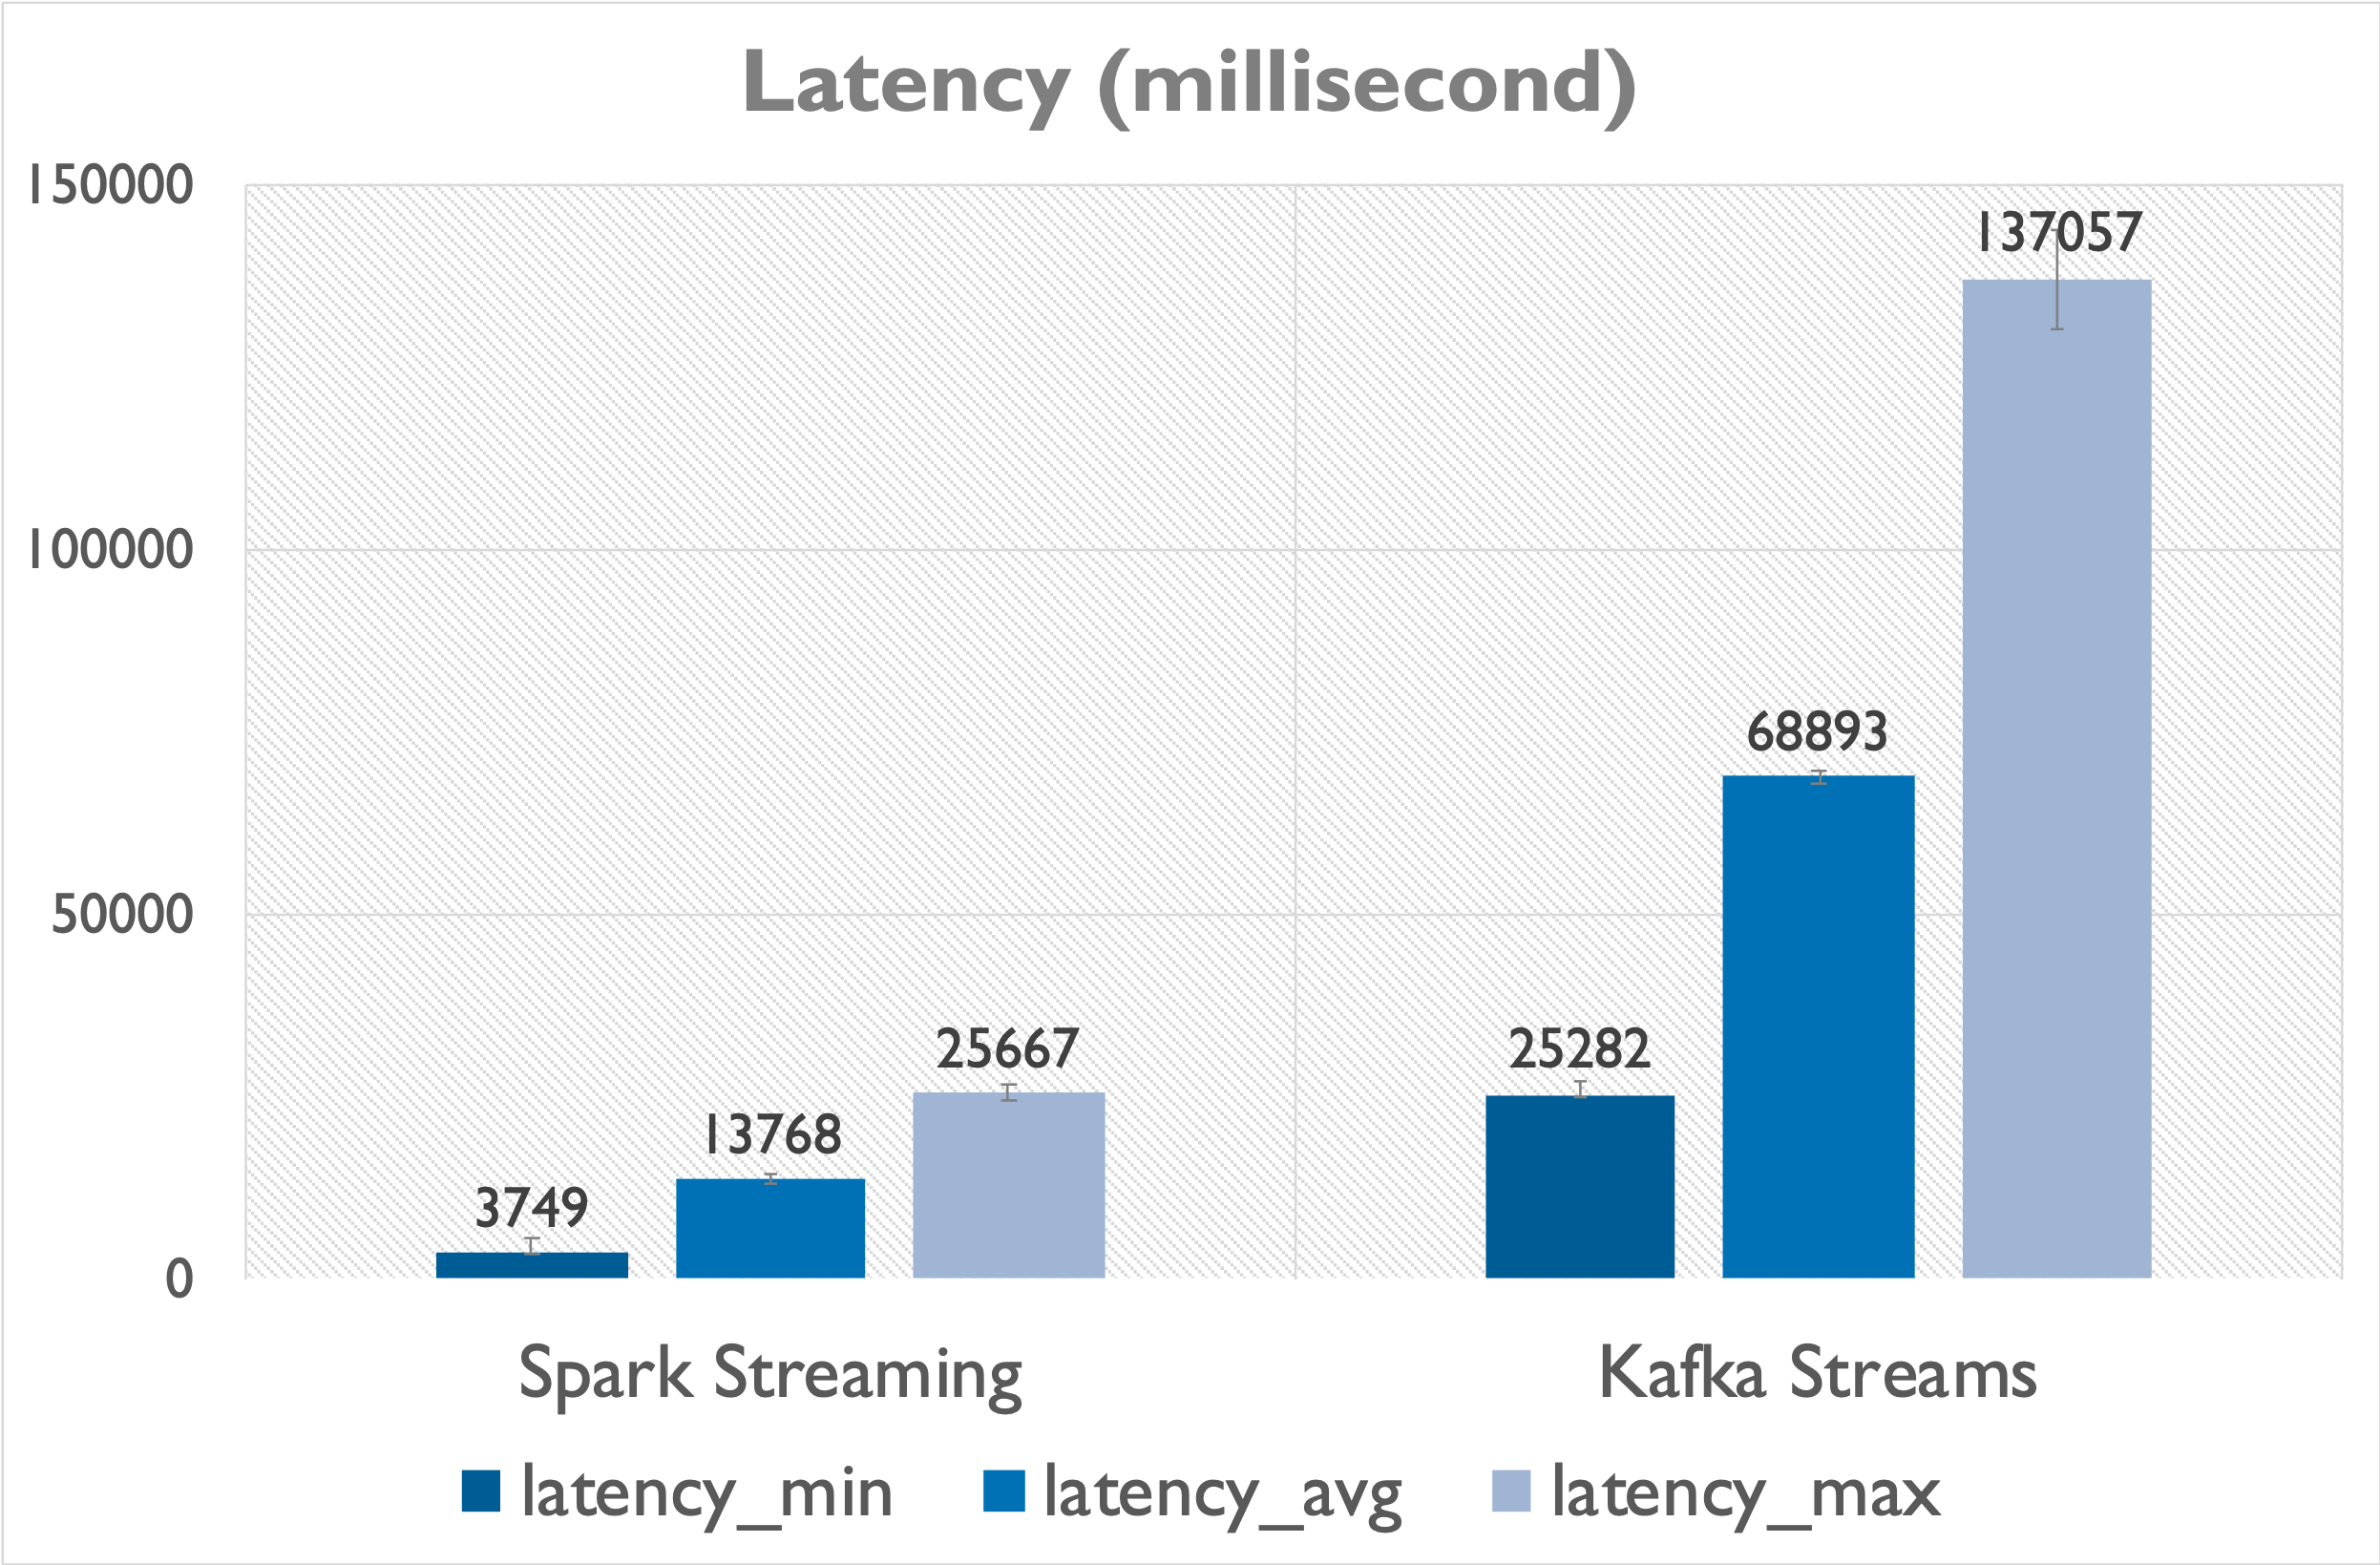
\includegraphics[width=\linewidth]{latency.png}
    \caption{Minimum, Average, and Maximum Latency of Spark Streaming and Kafka Streams}
    \label{fig:latency}
\end{figure}

\begin{figure}
    \centering
    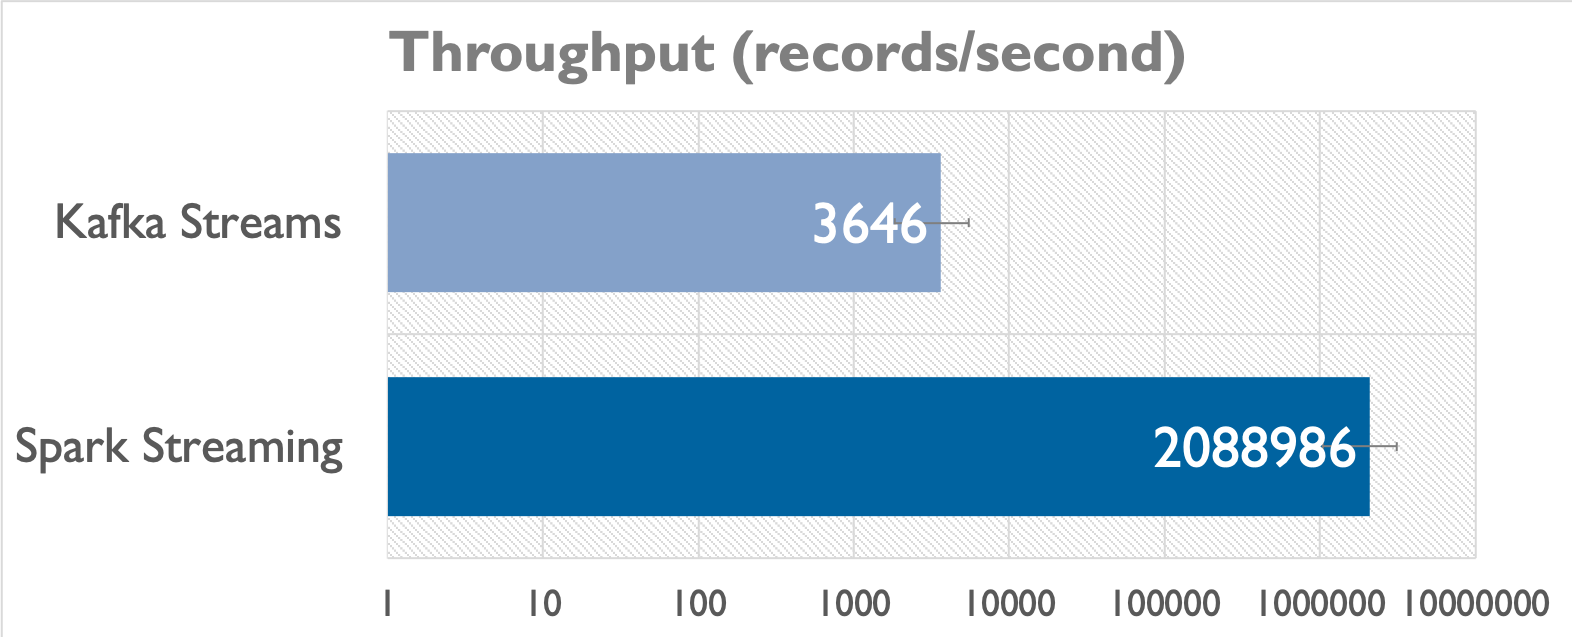
\includegraphics[width=\linewidth]{throughput.png}
    \caption{Throughput of Spark Streaming and Kafka Streams}
    \label{fig:throughput}
\end{figure}


The throughput was denoted by the average number of records in the processing duration. As shown in Figure \ref{fig:throughput}, the throughput in Spark Streaming achieved 2M/s, which completely outperformed Kafka streams. This is because Kafka Streams processes data as soon as they arrive while Spark Streaming treat stream data as micro-batches. With the use of micro-batches, data that arrive at approximately the same time can be grouped and processed together, which effectively increases the throughput. Therefore, Spark Streaming can process much more data at simultaneously than Kafka Streams can do, which is what we see in Figure \ref{fig:throughput}. 

\section{Conclusions}
The comparison among streaming data processing systems has become popular topics, and it is hard to pick an omnipotent data streaming platform because each of them studied here have their advantages and disadvantages. In addition to past traditional comparative research of data streaming systems that focused on performance benchmark of throughput and latency, we highlight the social factors in our report. These social factors, such as, are equally important as the performance because they reveal how active the relative communities are

We look forward to expanding this benchmark and testing newer releases of these systems as they come out.


{
    \bibliographystyle{ieeetr}
    \bibliography{ref}
}
\end{document}
